\documentclass[thesis.tex]{subfiles}

\title{Estimating duration in the presence of misclassification}
\author{Joshua Blake}
\date{\today}

\begin{document}

\ifSubfilesClassLoaded{
  \setcounter{chapter}{5}
}

\chapter{Survival analysis with false negatives} \label{imperf-test}

In \cref{E-perf-test}, a framework for analysing the CIS to produce estimates of the duration of positivity was developed.
However, initial application of this framework produced implausibly short estimates; I identified the issue as being due to the presence of false negatives, a form of misclassification bias, within the CIS (\cref{imperf-test:sec:problem}).
There exists little prior work on the incorporation of misclassification bias within similar survival analysis frameworks.
\todo[inline]{Review literature properly, here or elsewhere}
In this chapter, I modify the previous model to include false negatives (\cref{imperf-test:sec:modelling}).
I show in simulation that this model will recover the duration distribution (\cref{imperf-test:sec:sim-study-results}) and apply it to the CIS data (\cref{imperf-test:sec:application}).
Finally, I discuss the results and further work in \cref{imperf-test:sec:discussion}.

\section{The problem} \label{imperf-test:sec:problem}

Applying the method of \cref{E-perf-test} to CIS data gives implausible estimates of the duration distribution (see \cref{imperf-test:fig:problem-cis-estimates}).
In particular, it estimated a much shorter duration of positivity than in \cref{E-ATACCC}, despite those estimates being much more reliable over the first 2--3 weeks.
\begin{figure}
  \centering 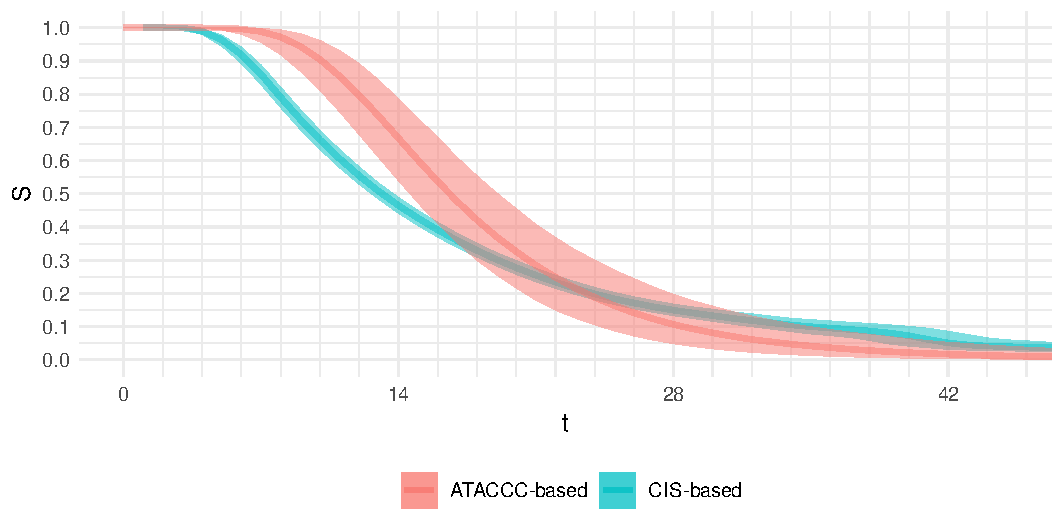
\includegraphics{cis-imperfect-testing/CIS_perfect}
  \caption[Estimating survival using CIS data assuming perfect testing]{Estimates of the survival function using CIS data alongside the ATACCC-based estimates of \cref{E-perf-test}. CIS-based is implausibly short over the first 14 days. \label{imperf-test:fig:problem-cis-estimates}}
\end{figure}

Comparing the simulated and CIS data suggests that this is due to the high frequency of single positive episodes in the CIS data.
A single positive episode is an episode containing exactly one positive test; intuitively, these cause short estimates because there is no lower bound on the length of time the episode lasts.
Furthermore, short episodes are very likely to be missed.
Therefore, there is little or no ability to upper bound the number of very short episodes.
I found that simulations building in even a few excess single positive episodes led to problematic estimation within the CIS setting (not shown).

\Textcite{shenNonparametrica}, extending \textcite{panNote}, studied the situation when only the terminating event is interval censored and the initiating event has simple left truncation.
This is related, although simpler, setting than the CIS; the CIS has double interval censoring and a more complex pattern of missed episodes (see \cref{E-perf-test:sec:problem}).
\Textcite{shenNonparametrica} showed that, in their situation, the maximum likelihood estimator is inconsistent and can lead to a severely biased underestimation of the survival function.
While the result cannot simply be extended to the more complex study design of the CIS, it reinforces the intuition that single positive episodes are likely to be problematic.

% Discussion and interrogation of the data led me to
I hypothesised that the reason for the unexpectedly high number of single positive episodes (compared to simulation) was the presence of false negatives results.
There are two strands of evidence supporting this hypothesis.
First, it is well known that PCR testing can return false negatives  (see \cref{E-biology-data:sec:PCR}); I explicitly include them in the viral load model of \cref{E-ATACCC}.
Intermittent negatives (described in  \cref{E-biology-data:sec:PCR}) show that they occur within the CIS.
Second, adjusting the simulation to include false negatives can reproduce both the CIS data more faithfully and exhibits the same issues when estimating the duration distribution (see \cref{imperf-test:fig:sim-single-pos}).
\begin{figure}
  \centering 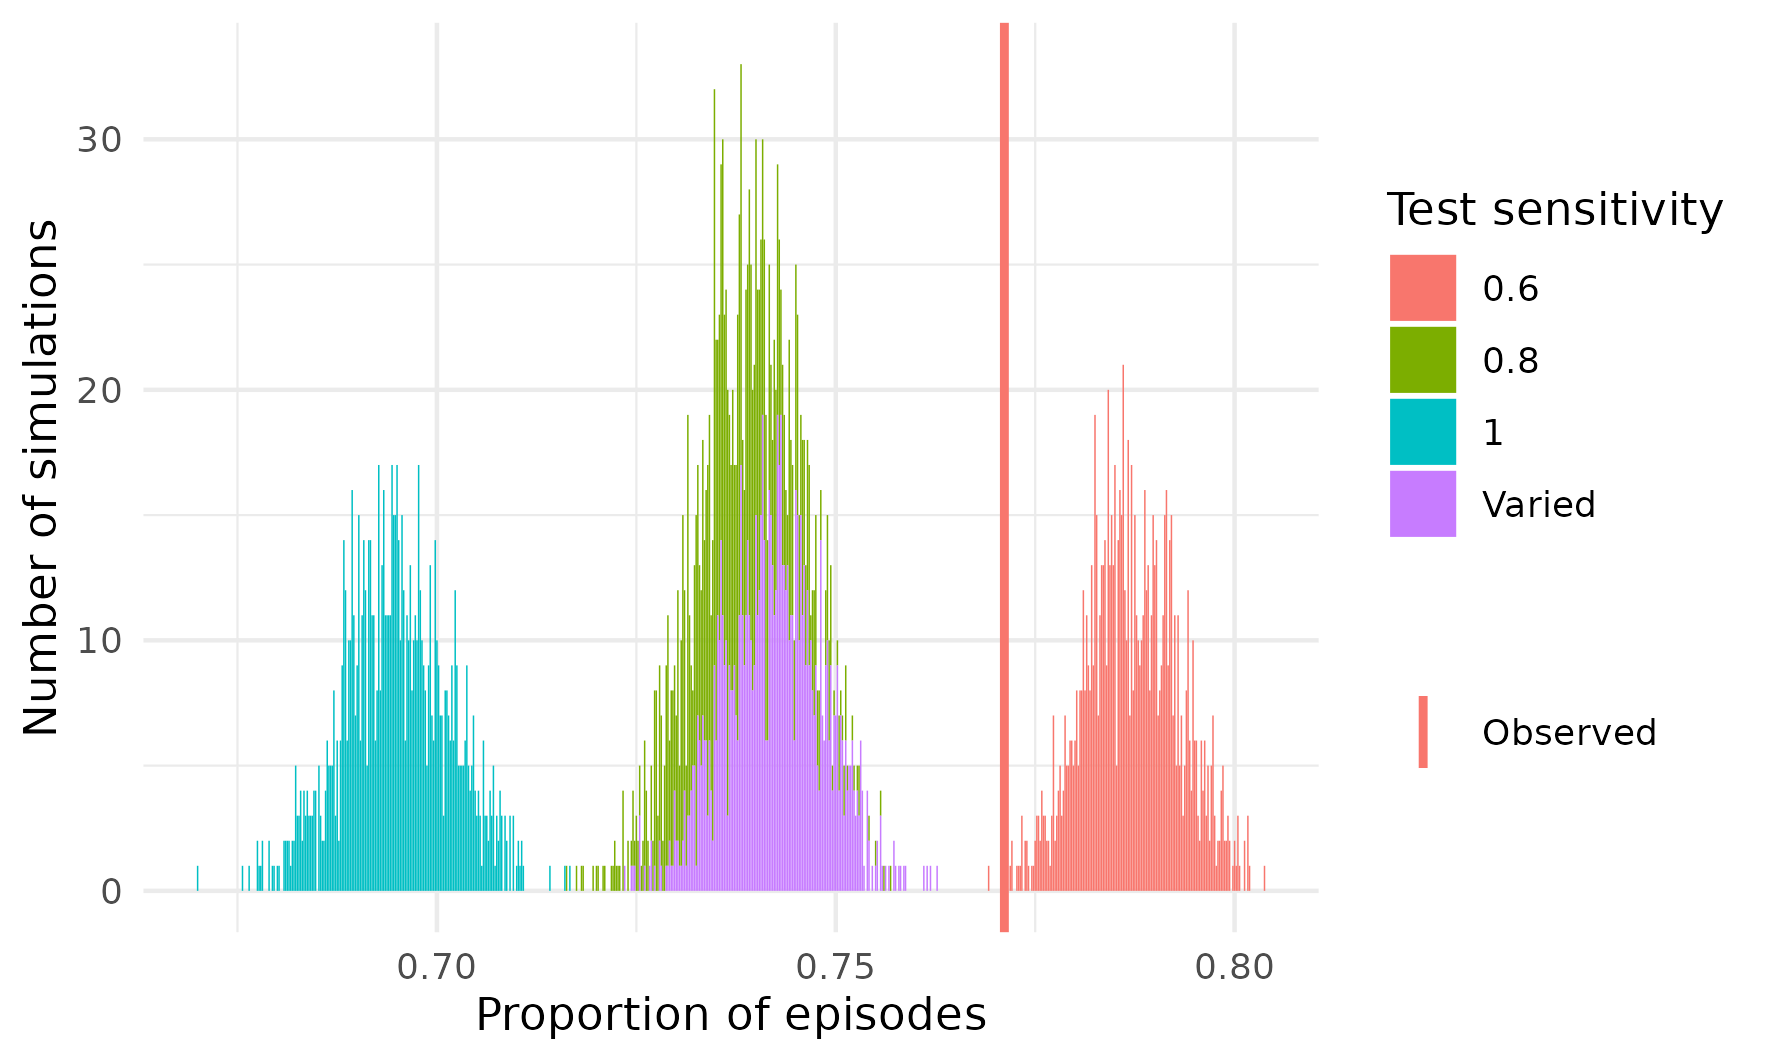
\includegraphics{cis-imperfect-testing/sim-single-positive-episodes}
  \caption[Single positive episodes in CIS simulation]{%
    Proportion of detected episodes which have a single positive episode.
    y-axis is the number of simulations, out of 1000, with the indicated proportion.
    The CIS data is shown as a vertical line.
    Simulation methodology is explained in \cref{E-perf-test:sec:simulation-study}, with false negatives included as described in \cref{imperf-test:sec:simulate}.
  }
  \label{imperf-test:fig:sim-single-pos}
\end{figure}

\section{Modelling false negatives} \label{imperf-test:sec:simulate}

The simplest model for false negatives is a constant probability of returning a negative test even when detectable.
The probability of testing positive given being detectable is known as the \emph{test sensitivity}, $\psens$.
$\psens = 1$ means that there are no false negatives, the situation previously considered.
False negatives are formalised by defining the outcome of a test as a random binary variable such that:
\begin{equation}
  \prob(Y_i(t) = 1) \begin{cases}
      \psens &b_i \leq t \leq e_i \\
      0 &\text{otherwise}
  \end{cases} 
\end{equation}
where $Y_i(t)$ is only defined for $t \in \sched_i$.
However, an implausibly low value for $\psens$ is required to reproduce the rate of single positive episodes seen in the CIS.

More plausibly, the rate of false negatives varies over the course of an episode.
False negatives are more likely to occur when the viral load of an individual is low, because there is less virus in their body to be sampled.
In \cref{E-ATACCC}, this mechanism is incorporated by the left-censored observations.
This suggests that a model with a declining test sensitivity as a function of time since infection might be more suitable.

The CIS data provides evidence for a test sensitivity declining over the course of an episode.
\Cref{imperf-test:fig:bounding-cis-sensitivity} demonstrates this by classifying all test results as follows.
\begin{enumerate}
    \item All positive results are true positives.
    \item All intermittent negatives are false negatives.
    \item The negative at the end of an episode is a possible false negative.
    \item All other negatives are true negatives.
\end{enumerate}
Here, I am assuming that the probability of two false negative tests at the end of an episode is negligible.
Then I calculate the test sensitivity as a function of days since the first positive in an episode, bounding this by assuming either all or none of those in group 3 are false negatives.
% The test sensitivity is the true positives / (true positives + false negatives).
% In \cref{imperf-test:fig:bounding-cis-sensitivity} we consider the values produced by assuming the negative following the last positive in an episode could be either a true or false negative as a function of time since the individual was detected (\ie: the first positive test in the episode).
This generates broad bounds, although suggest a declining test sensitivity over the course of an episode.
\begin{figure}
  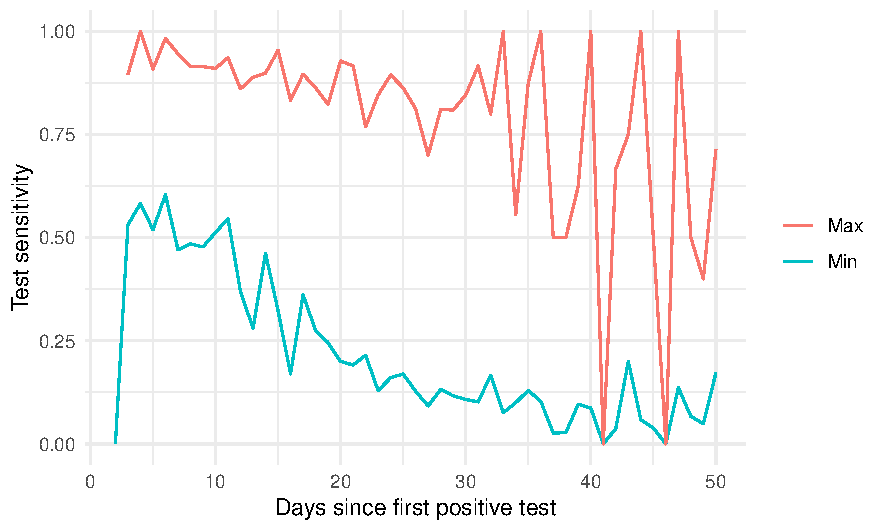
\includegraphics{cis-imperfect-testing/test-sens-bound}
  \caption[Bounding test sensitivity using CIS data]{
    Bounding the test sensitivity using CIS data as a function of time since the infection was detected (see main text for explanation of how the bounds are formed).
    Small numbers of tests mean that the series is noisy near the start and the end.
  }
  \label{imperf-test:fig:bounding-cis-sensitivity}
\end{figure}

Based on \cref{imperf-test:fig:bounding-cis-sensitivity}, I propose the following model for test sensitivity, consisting of a linearly declining period then a constant period:
\begin{equation}
  p_\text{sens}(t) = \begin{cases}
    0.9 - \frac{0.9-0.5}{50}t &t \leq 50 \\
    0.5 &t > 50
  \end{cases}
  \label{imperf-test:eq:variable-test-sensitivity}
\end{equation}
where $t$ is the time in days since infection.
Simulated data using this test sensitivity is much more similar to the data (see \cref{imperf-test:fig:sim-single-pos}), while being more plausible than very low probabilities of false negatives.

\section{Modelling} \label{imperf-test:sec:modelling}

In this section, I introduce a simple model of false negatives into the model of \cref{E-perf-test:sec:model}.
A simple model means that the likelihood remains tractable.
I modify both $p_{ia}$ to allow for the episode possibly being longer than observed (\cref{imperf-test:sec:modifying-p_ia}), and $p_{iu}$ (\cref{imperf-test:sec:modifying-p_iu}) to allow for additional episodes being missed.

A constant test sensitivity is assumed throughout this section.
Further work is required to introduce the more realistic assumption of declining test sensitivity over the course of an episode.

\subsection{Modifying \texorpdfstring{$p_{ia}$}{pia}} \label{imperf-test:sec:modifying-p_ia}

I modify $p_{ia}$ to allow the negative test following the last positive to be a false negative.
If it is a false negative, then we consider the episode's length right-censored.
However, if it is in fact a true negative, then we are in the same case as before with a bound on the length of the episode.
A mixture of these scenarios then forms the episode's likelihood contribution, with the mixture probability determined by the test sensitivity.

For tractability, assume that the negative test bounding the start of the infection, at $l_i^{(b)}-1$, is a true negative.
This assumption is reasonable because the test sensitivity is high early in an infection, therefore this test is unlikely to be a false negative.
Consider only the tests between $r_i^{(b)}$ and $l_i^{(e)}$ inclusive (the positive tests providing a lower bound on the length of the episode).
Denote these tests by $\sched'_i = \{ t \in \sched_i : r_i^{(b)} \leq t \leq l_i^{(e)} \}$ and their results by $y_i'$.
The test results at times in $\sched_i'$ are either true positives or false negatives. 
By definition, the test at $r_i^{(e)}$ is a false negative if and only if $e_i > r_i^{(e)}$.
I proceed by considering whether this is the case.

First, if $e_i \leq r_i^{(e)}$.
In this case, the test at $r_i^{(e)}$ is a true negative, as are all other tests not in $\sched'_i$.
These occur with probability 1, as I continue to assume no false positives.
\begin{align}
&p(y_i', e_i \leq r_i^{(e)} | b_i, p_\text{sens}, \theta) \\
&= p(y_i', l_i^{(e)} \leq e_i \leq r_i^{(e)} | t_i, b_i, p_\text{sens}, \theta) \\ % &\text{as no false positives}
&= p(y_i' \mid l_i^{(e)} \leq e_i \leq r_i^{(e)}, t_i, b_i, p_\text{sens}, \theta) p(l_i^{(e)} \leq e_i \leq r_i^{(e)} | t_i, b_i, p_\text{sens}, \theta) \\
&= \left( \prod_{t \in \sched'_i} p_\text{sens}^{y_i(t)} (1 - p_\text{sens})^{(1 - y_i(t))} \right) \left( S_\theta(l_i^{(e)} - b_i - 1) - S_\theta(r_i^{(e)} - b_i - 1) \right)
\end{align}

Second, if $e_i > r_i^{(e)}$.
In this case, the test at $r_i^{(e)}$ is a false negative, occurring with probability $(1 - p_\text{sens})$, and the end of the infection is right-censored.
\begin{align}
&p(y_i', e_i > r_i^{(e)} | b_i, p_\text{sens}, \theta) \\
&= p(y_i \mid e_i > r_i^{(e)}, t_i, b_i, p_\text{sens}, \theta) p(e_i > r_i^{(e)} | t_i, b_i, p_\text{sens}, \theta) \\
&= \left( \prod_{t \in \sched'_i} p_\text{sens}^{y_i(t)} (1 - p_\text{sens})^{(1 - y_i(t))} \right) (1 - p_\text{sens}) S_\theta(r_i^{(e)} - b_i - 1)
\end{align}

Combining the above, the replacement for $p_{ia}$ is:
\begin{align}
p_{ia}'
&= p(y_i' \mid p_\text{sens}, \theta) \\
&= \sum_{b_i = l_i^{(b)}}^{r_i^{(b)}} \left( p(y_i', b_i, e_i \leq r_i^{(e)} \mid p_\text{sens}, \theta) p(y_i', b_i e_i > r_i^{(e)} \mid p_\text{sens}, \theta) \right) p(b_i \mid p_\text{sens}, \theta) \\
&= \left( \prod_{t \in \sched'_i} p_\text{sens}^{y_i(t)} (1 - p_\text{sens})^{(1 - y_i(t))} \right) \\ & \ \times \sum_{b_i = l_i^{(b)}}^{r_i^{(b)}} \left( S_\theta(l_i^{(e)} - b_i - 1) - S_\theta(r_i^{(e)} - b_i - 1) + (1 - p_\text{sens}) S_\theta(r_i^{(e)} - b_i - 1) \right) \\ & \ \times p(b_i \mid p_\text{sens}, \theta) \\
&= \left( \prod_{t \in \sched'_i} p_\text{sens}^{y_i(t)} (1 - p_\text{sens})^{(1 - y_i(t))} \right) \\ & \ \times \sum_{b_i = l_i^{(b)}}^{r_i^{(b)}} \left( S_\theta(l_i^{(e)} - b_i - 1) - p_\text{sens} S_\theta(r_i^{(e)} - b_i - 1) \right) p(b_i \mid p_\text{sens}, \theta).
\label{imperf-test:eq:pia-prime}
\end{align}
Note that if $p_\text{sens} = 1$ then $p_{ia}' = p_{ia}$.

\subsection{Modifying \texorpdfstring{$p_{iu}$}{piu}} \label{imperf-test:sec:modifying-p_iu}

With false negatives, an episode with can be undetected in the following four ways; the first two of these are the same as before, but the second two are new.
Note that each of these is mutually exclusive.
\begin{enumerate}
\item
  The episode begins before the individual's first test: $b_i \leq \min \sched_i$.
  % I assume there is a negligible probability of a false negative test at this point because viral load is high.
\item
  The episode begins after the individual's first test, but ends before the next test after beginning: $b_i \leq \min \sched_i$ and $e_i < b_i + \tau_{\sched_i}(b_i)$.
\item
  The episode begins after the individual's first test, ends after the first test at or following $b_i$, that test is a false negative, but the episode ends before the second test at or following $b_i$.
  Then, $D_i$ of the episode is greater than $\tau_{\sched_i}(b_i)$ less than  $\tau^2_{\sched_i}(b_i) \stackrel{\text{def}}{=} \tau_{\sched_i}(\tau_{\sched_i}(b_i) + 1)$, and a false negative episode occurred at the first test after $t$.
  This probability, conditional on $b_i$ is:
  \begin{align}
    &\prob \left( b_i + \tau_{\sched_i}(b_i) \leq E_i < b_i + \tau^2_{\sched_i}(b_i), Y_i(b_i + \tau_{\sched_i}(b_i) = 0) \mid b_i, \theta \right) \\
    &= \prob \left(\tau_{\sched_i}(b_i) + 1 \leq D_i < \tau^2_{\sched_i}(b_i) + 1 \mid b_i, \theta \right) (1 - \psens) \\
    &= \left( S_\theta(\tau_{\sched_i}(b_i) + 1) - S_\theta(\tau^2_{\sched_i}(b_i) + 1) \right) (1 - \psens).
  \end{align}
  Integrating over $b_i$ for $b_i > \min \sched_i$, in the same way as \cref{E-perf-test:eq:piu}, gives:
  \begin{align}
    (1 - p_\text{sens})\frac{1}{T} \sum_{b=\min(\sched_i)}^T \left( S_\theta(\tau_{\sched_i}(b) + 1) - S_\theta(\tau^2_{\sched_i}(b) + 1) \right).
  \end{align}
\item
  The episode begins after the individual's first test, ends after the second test at or following $b_i$, and all tests within the episode (at least two) are false negatives.
  I assume this occurs with negligible probability.
\end{enumerate}

Therefore, $p_{iu}$ is replaced by $p_{iu}'$, the sum of: $p_{iu}$ (for number 1 and 2; derived in \cref{E-perf-test:eq:piu}), and the probability in number 3.
For the posterior density (\cref{E-perf-test:eq:full-posterior}), $1 - p_{iu}'$ is the required quantity:
\begin{align}
1 - p_{iu}'
&= 1 - p_{iu} - (1 - p_\text{sens})\frac{1}{T} \sum_{b=\min(t_i)}^T \left( S_\theta(\tau_{\sched_i}(b) + 1) - S_\theta(\tau^2_{\sched_i}(b) + 1) \right) \\
&= \frac{1}{T} \sum_{b=\min(t_i)}^T \left( p_\text{sens} S_\theta(\tau_{\sched_i}(b) + 1) + (1 - p_\text{sens}) S_\theta(\tau^2_{\sched_i}(b) + 1)\right).
\label{imperf-test:eq:pit-prime}
\end{align}

$p_{iu}'$ and $p_{ia}'$ are substituted for $p_{iu}$ and $p_{ia}$ respectively in \cref{E-perf-test:eq:full-posterior}.
The posterior density is otherwise unchanged.

\section{Simulation study} \label{imperf-test:sec:sim-study-results}

I repeated the simulation study in \cref{E-perf-test:sec:simulation-study}, except I used the model of \cref{imperf-test:sec:modelling} with either a constant test sensitivity or the more realistic varying sensitivity.
I focus on the independent (vague) and model combination priors for the survival (described in \cref{E-perf-test:sec:parameters-priors}.
These were shown to be the best performing priors in \cref{E-perf-test:sec:results}.

With a constant test sensitivity of 0.8, the model recovers the true survival time well.
However, with a lower test sensitivity of 0.6, this is no longer the case (see \cref{imperf-test:fig:constant-test-sensitivity}).
The simplifications to the model made in \cref{imperf-test:sec:modelling} cause too large a misspecification at this point.
The informative prior helps to overcome the misspecification, helping to recover the true survival time (in comparison to the vague prior).
\begin{figure}
  % \makebox[\textwidth][c]{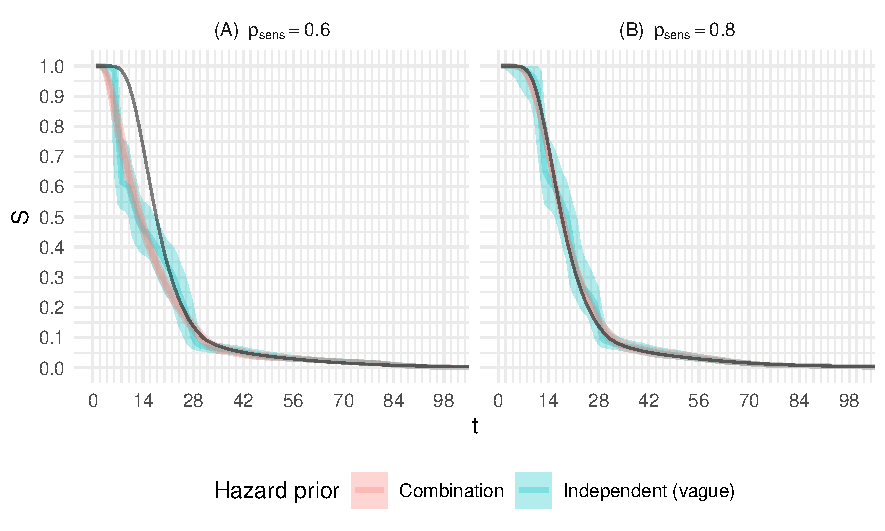
\includegraphics[width=1.2\textwidth]{cis-imperfect-testing/sim-constant-sensitivity}}
  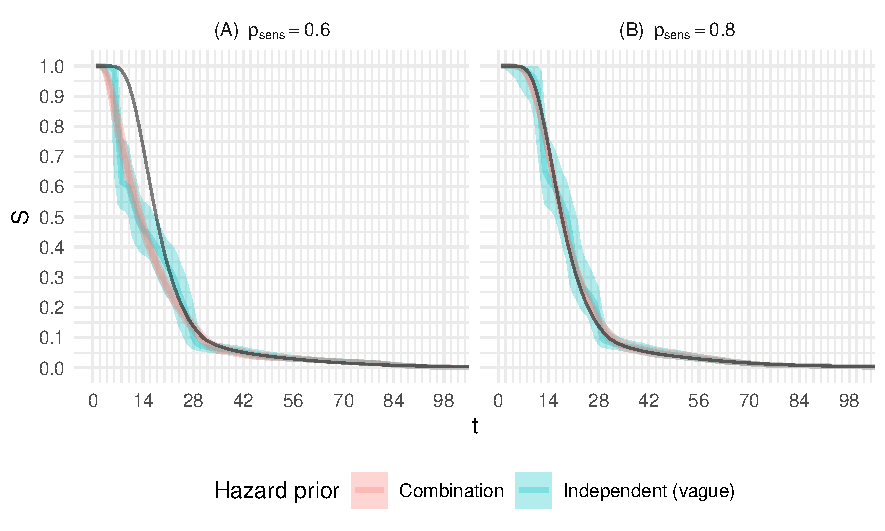
\includegraphics[width=\textwidth]{cis-imperfect-testing/sim-constant-sensitivity}
  \caption[Simulation study results with constant test sensitivity]{%
    Posterior (median and 95\% credible interval) of the survival time for the simulation study with a constant test sensitivity.
    True survival time shown in black.
    Left panel shows the results with a test sensitivity of 0.6, right panel shows the results with a test sensitivity of 0.8.
  }
  \label{imperf-test:fig:constant-test-sensitivity}
\end{figure}

If the test sensitivity is misspecified, that is the assumed value for $p_\text{sens}$ in \cref{imperf-test:eq:pit-prime,imperf-test:eq:pit-prime} is different to the value used in the simulation, then the survival time will be biased (see \cref{imperf-test:fig:misspecified-test-sensitivity}).
If the test sensitivity is assumed to be too low, then the number of episodes inferred to have truly ended by the first negative will be too high, and the survival time will be underestimated.
This affect dominates over the opposing bias of overestimating the number of missed episodes.
The opposite occurs if the test sensitivity is assumed to be too high.
\begin{figure}
  % \makebox[\textwidth][c]{
    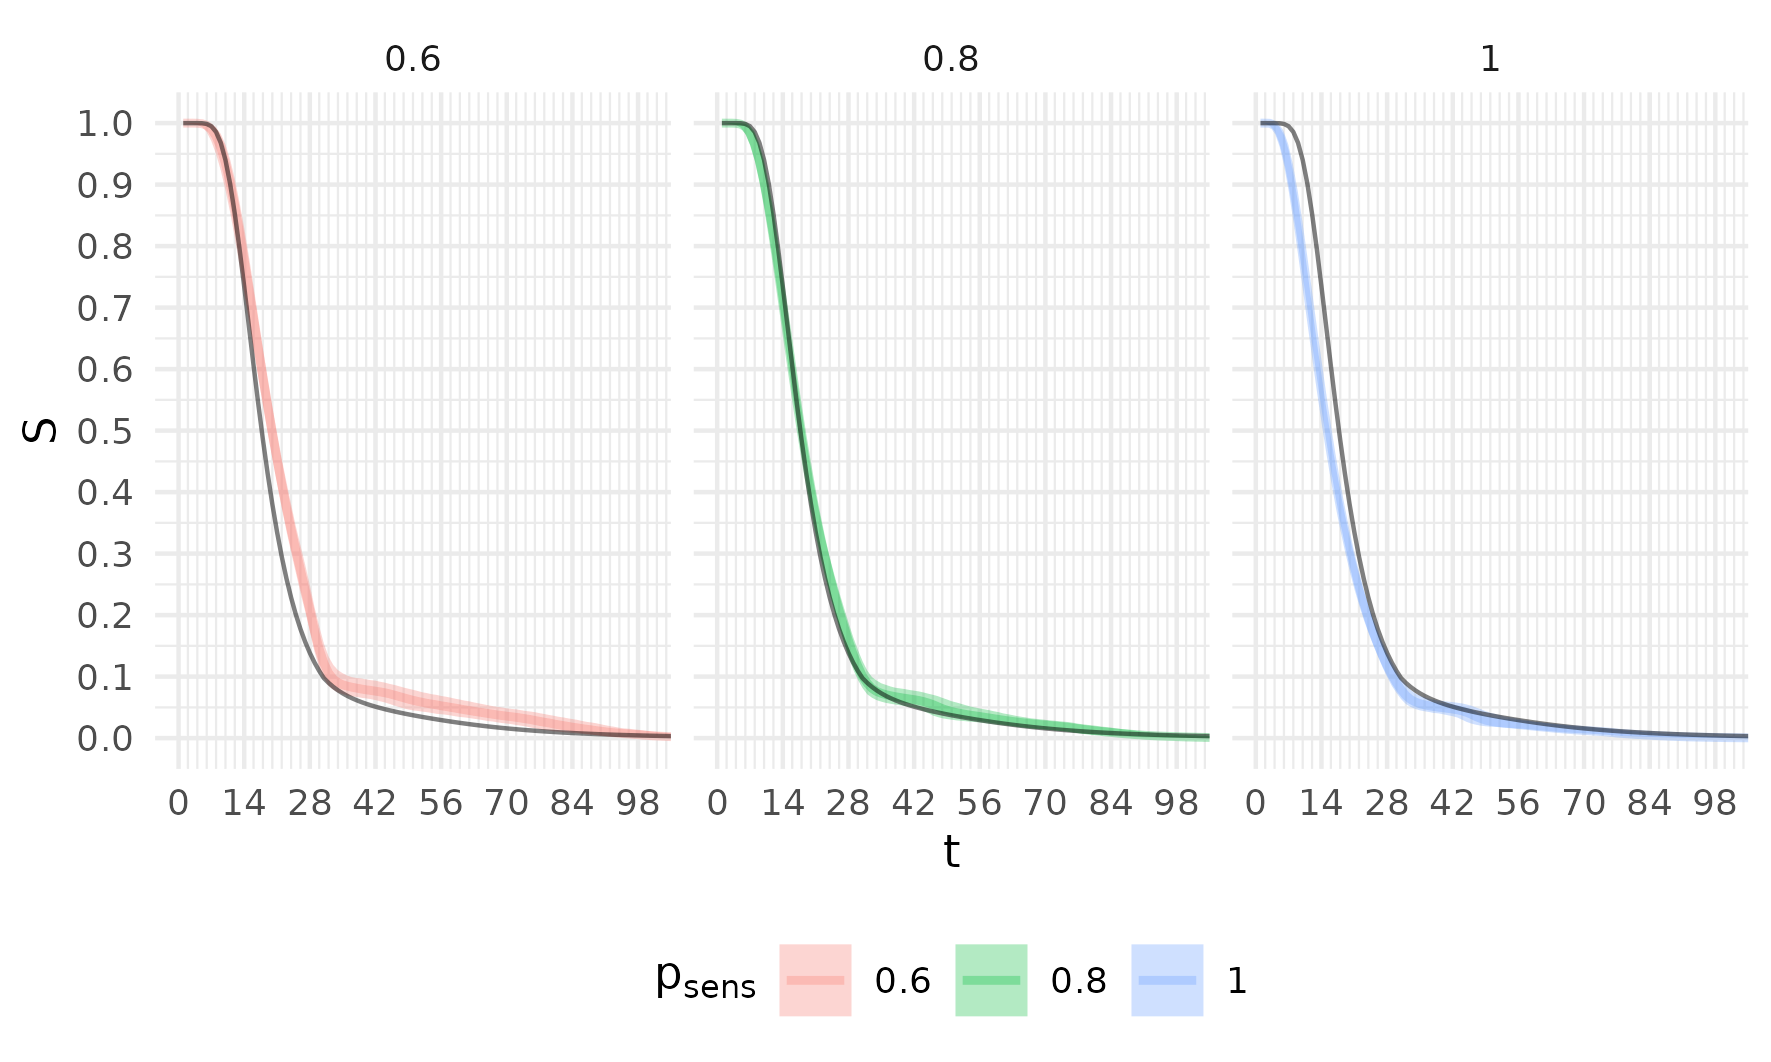
\includegraphics[width=\textwidth]{cis-imperfect-testing/sim-misspecified-sensitivity}
  \caption[Simulation study results with misspecified test sensitivity]{%
    Posterior (median and 95\% credible interval) of the survival time for the simulation study with a misspecified test sensitivity.
    True survival time shown in black.
    All simulations use a constant test sensitivity of 0.8, but the model assumes different values.
    All inference uses the combination prior, due to it performing better than the vague prior in \cref{imperf-test:fig:constant-test-sensitivity}.
    The correctly specified model (middle pane) has a posterior median closely following the true value, with the credible intervals almost always including the true value.
    Assuming a too low test sensitivity (left pane) starts by following the true value but then separates, with the posterior median being too high.
    Assuming a too high (perfect) test sensitivity (right pane) underestimates the survival time almost throughout.
  }
  \label{imperf-test:fig:misspecified-test-sensitivity}
\end{figure}

The results when a varying test sensitivity (\cref{imperf-test:eq:variable-test-sensitivity}) is used for the simulation are similar to a constant 0.8 test sensitivity (see \cref{imperf-test:fig:variable-test-sensitivity}).
This suggests that the simplified model, with constant test sensitivity, is sufficient for recovering the true survival time.
Therefore, I will apply this model to the real CIS data in the next section.
\begin{figure}
  % \makebox[\textwidth][c]{
    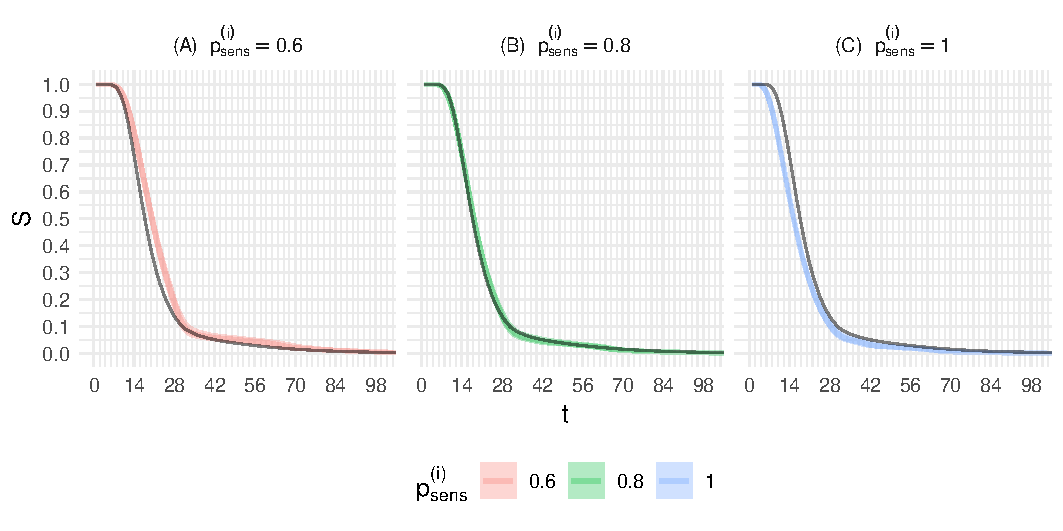
\includegraphics[width=\textwidth]{cis-imperfect-testing/sim-variable-sensitivity}
  \caption[Simulation study results with varying test sensitivity]{%
    Posterior (median and 95\% credible interval) of the survival time for the simulation study with a variable test sensitivity.
    Each panel shows the results of performing inference with a different assumed value for the test sensitivity.
    The posterior estimate using a model with a constant test sensitivity of 0.8 (middle panel) is similar to the true value (black line).
  }
  \label{imperf-test:fig:variable-test-sensitivity}
\end{figure}

\section{Application to CIS data} \label{imperf-test:sec:application}

This section applies the model described in this chapter to the CIS episodes dataset I described in \cref{E-perf-test:sec:approach}.

Unlike in the simulation studies, an uninformative prior on $\ntot$ led to implausible estimates of the duration distribution.
The uninformative prior led to high posterior estimates of $\ntot$, and hence an implausibly large number of episodes with durations of less than five days.
Therefore, I based an informative prior for $\ntot$ on pre-existing estimates of the total number of infections over the period with posterior mean \numprint{4136368} and standard deviation \numprint{27932}~\autocite{birrellRTM2}.
% This model gives a posterior mean of \numprint{4136368} cumulative infections in England in the time period I consider, with a posterior standard deviation of \numprint{27932}~\citePersonalComms{Paul Birrell}.
\todo{Insert correct citation for RTM paper 2 once available}
Approximating this distribution as a negative binomial and scaling the mean to the size f the CIS cohort gives the prior $\ntot \sim \NBc(\numprint{25132}, \numprint{22047})$.

With this prior, the model produces plausible estimates of the duration distribution (see \cref{imperf-test:fig:cis-estimates}).
This estimate has more long episodes than the estimate in \cref{E-ATACCC}.
The qualitative increase in long episodes is robust to the choice of prior for $\ntot$, the assumed value for $\psens$ (see \cref{imperf-test:fig:cis-sensitivity}), and the choice of prior for $\lambda$.
However, the survival proportion over the first 4 weeks is sensitive to these choices.
The estimate using a test sensitivity of 0.8 and $\NBc(\numprint{25132}, \numprint{22047})$ give a median survival time most similar to that of \cref{E-ATACCC}.
\begin{figure}
  \centering 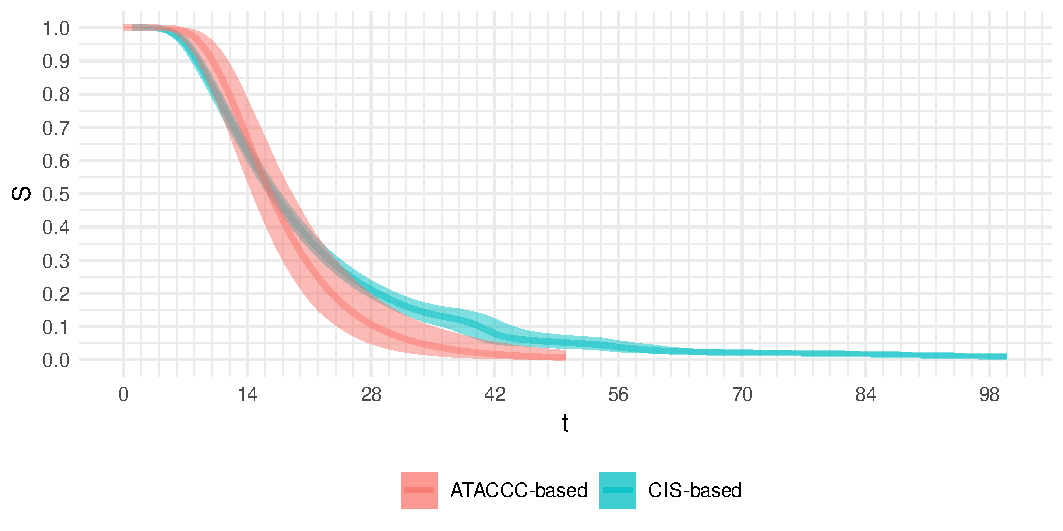
\includegraphics{cis-imperfect-testing/CIS_final}
  \caption{Duration estimates using CIS and ATACCC data}
  \label{imperf-test:fig:cis-estimates}
\end{figure}
\begin{figure}
  \vspace{-2.5cm}
  \makebox[\textwidth][c]{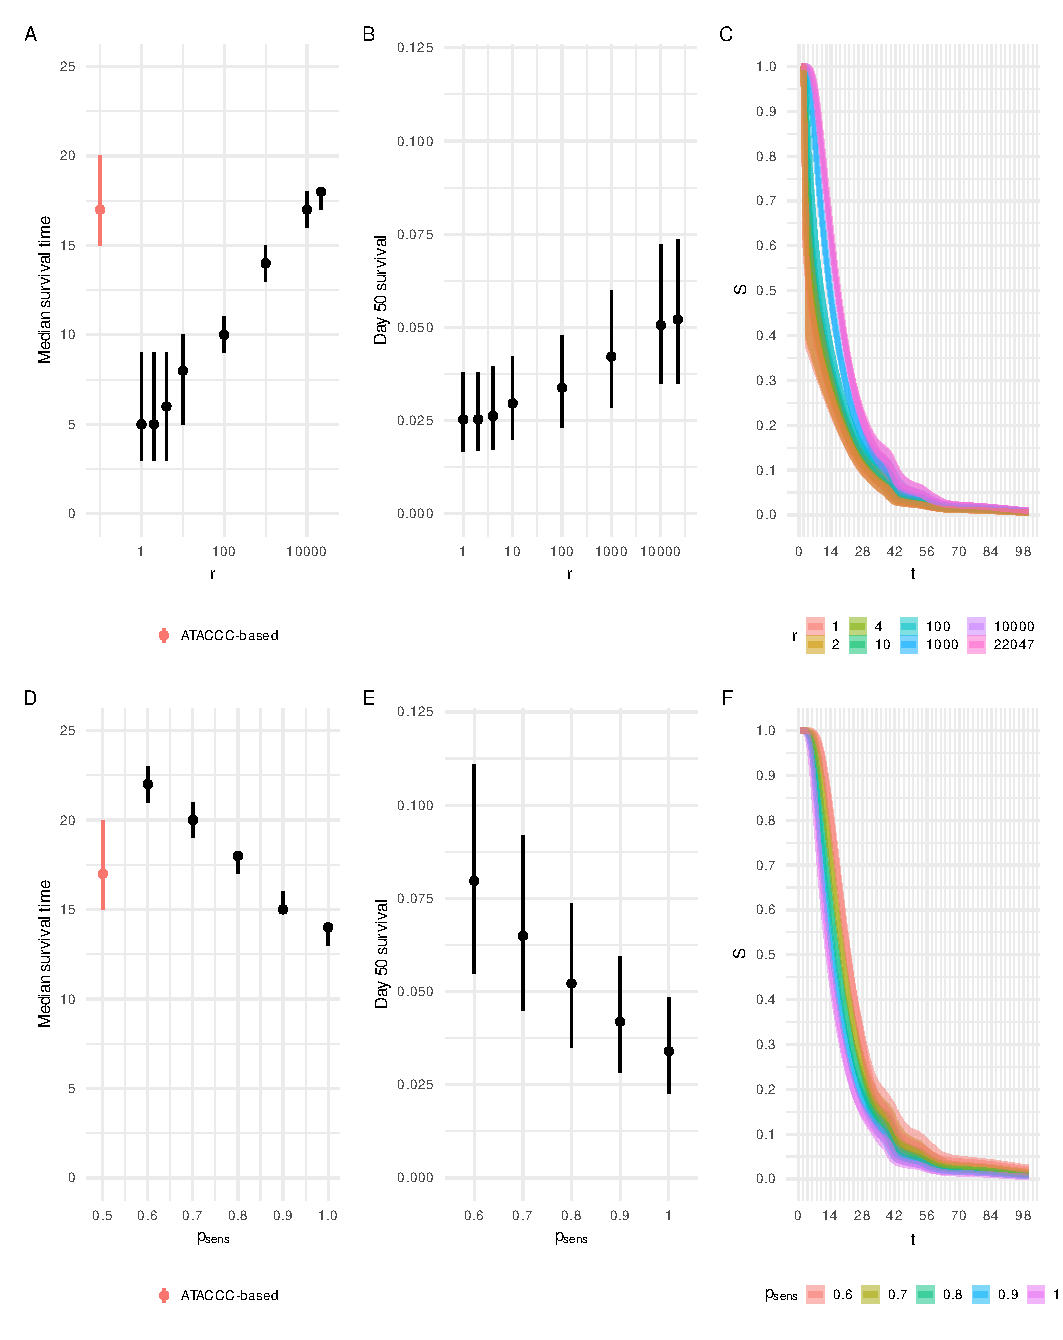
\includegraphics{cis-imperfect-testing/CIS_vary}}
  \caption{%
    Sensitivity of CIS estimates to: (A-C) the value of $r$ in the prior for $\ntot$ and (D-F) $\psens$.
    A and D: median survival time, in comparison to the ATACCC-based estimate of \cref{E-ATACCC}.
    B and E: survival at day 50, $S_\theta(50)$.
    C and F: full survival curves out to day 100.
  }
  \label{imperf-test:fig:cis-sensitivity}
\end{figure}

The assumption that the estimates are most sensitive to is the strength of the prior on $\ntot$.
A very weak, almost uninformative, prior on this quantity causes the posterior estimate to be much higher than the estimate from \textcite{birrellRTM2}.
When increasing the prior's strength, the posterior estimate moves towards the prior smoothly, as expected (see \cref{imperf-test:fig:ntot}).
Taking a prior from \textcite{birrellRTM2} means that the posterior survival is close to the \cref{E-ATACCC} estimate in the region where that estimate is reliable.
This justifies the use of this prior.
\begin{figure}
  \centering 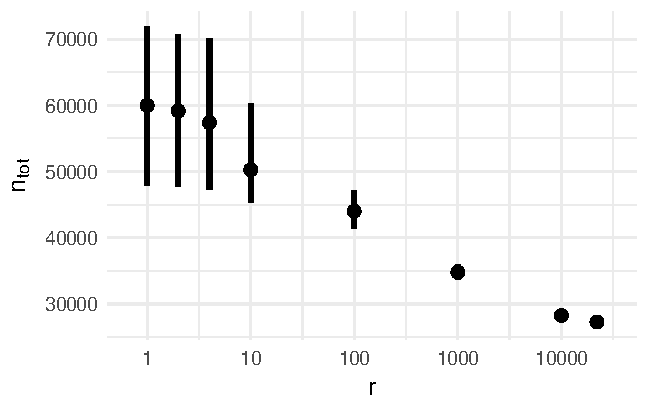
\includegraphics{cis-imperfect-testing/CIS_ntot}
  \caption{How the posterior estimate of $\ntot$ changes with the value of $r$ in the prior on $\ntot$.}
  \label{imperf-test:fig:ntot}
\end{figure}

\section{Discussion} \label{imperf-test:sec:discussion}

% \begin{itemize}
%   \item Survival prior matters for quantitative details but not qualitative shape. 
%   \item Number of missed infections prior is more important, but not the case in simulation (not shown).
%   \item Unclear why this is the case, probably model misspecification meaning that fewer missed infections than expected.
%   \item Two possible misspecifications: test sensitivity (not constant) and constant incidence.
% \end{itemize}

This chapter shows that a simple model of false negatives can be incorporated into the model of \cref{E-perf-test}.
This model allows estimation of the duration distribution tails without the strong model assumptions used in \cref{E-ATACCC}.
The qualitative features of the estimated distribution are robust to the assumed value for $\psens$, and the choice of prior for $\lambda$, although the quantitative details are not.
The estimates of the tail, the primary purpose of this chapter, are in addition robust to the choice of prior for $\ntot$.
However, the rest of the distribution is sensitive to this choice.

An informative prior on $\ntot$ is required is for the bulk of the distribution to be plausible.
In the simulation study, the uninformative prior on $\ntot$ performed well, even when the test sensitivity was misspecified.
One hypothesis is that the test sensitivity is significantly different to the function in \cref{imperf-test:eq:variable-test-sensitivity} causing an unintuitive pattern of results.
In particular, the test sensitivity for long episodes may become much lower than 50\%.
This allows many more episodes to be missed than the model assumes, and hence a higher $\ntot$ is required to explain the data.
Furthermore, it violates assumptions made in \cref{imperf-test:sec:modelling}; this is similar to when the simulating using a too low test sensitivity.
Violating these assumptions would lead to unpredictable inference results, perhaps those seen here.

Ideally, the test sensitivity would be estimated from the data.
However, this would require a model for time-varying test sensitivity to be incorporated into the model.
Furthermore, it is unclear that such a model would be identifiable because it would not be clear whether to attribute negative results to false negatives or to recoveries\todo{cite identifiability issues with varying sensitivity}.

The assumption, made in \cref{E-perf-test}, was that the episode start times are independent.
However, because infections are the result of a counting process with intensity shared between individuals (see \cref{E-inc-prev:sec:infection-process}), this assumption is violated.
Prevalence was fairly constant over the period I chose, suggesting the same is true of the incidence.
Additionally, some simulations exploring the results of changing incidence suggested this would not have a large effect on the results (not shown).

% However, comparing the CIS and simulated datasets do not show any differences which suggest what in the data is causing these differences.
% Then, the additional missed infections implied by a 
% This would lead to more missed infections than the model assumes, and hence a higher $\ntot$ is required to explain the data.

\section{Conclusion} \label{imperf-test:sec:conclusion}

This chapter has produced estimates of the duration distribution of PCR-positivity using information from two studies: ATACCC and CIS.
Assuming a test sensitivity of 0.8 and an informative prior on the number of infections, provided the preferred estimates.

These estimates are the first estimates of the duration of PCR-positivity, including the distribution tails, estimated from general population data.
This feature of the distribution is important for understanding the proportion of prevalence attributable to long infections and interpreting PCR test results.
Producing these estimates required applying previous survival analysis frameworks in the novel context of the CIS.
The framework needed further modification to account for the presence of false negatives, done in this chapter.

The posterior distribution for the survival is concentrated, producing narrow credible intervals.
In the following chapters, I will take the posterior mean for the survival time at each point, neglecting this uncertainty, as the basis for estimating transmission.
First, I will take a backcalculation approach (\cref{E-backcalc}), based on the framework in \cref{E-inc-prev}.
Then, I will take a mechanistic approach (\cref{E-SEIR}), modelling the transmission process explicitly.

\ifSubfilesClassLoaded{
  \listoftodos
}{}

\end{document}